\documentclass[a4paper]{article} \usepackage[backend=biber, style=numeric, sorting=none]{biblatex}
\usepackage[a4paper, left=0.8cm, right=0.8cm, top=0.8cm, bottom=0.8cm, landscape]{geometry}
% \usepackage{showframe}
\usepackage{multicol}
\usepackage{blindtext}
\usepackage{listings}
\usepackage{graphicx}
\usepackage{enumitem}
\graphicspath{{images/cs2105/}}

\begin{document}
\setlength\parindent{0pt} %TODO this somehow messes up paragraph vertical spacing as well?
\scriptsize
% \tiny
\pagenumbering{gobble}

\begin{center}
{\large CS2105 Cheatsheet 18/19 S1 Midterms}\\
\end{center}
    \begin{multicols*}{4}

% APPLICATION LAYER %
{\small\textbf{Application Layer}} \\
\textbf{Processes}
\begin{itemize}[leftmargin=*]
\itemsep -0.5em
\item Applications send \texttt{messages} to each other using \texttt{sockets}
\item Application processes can only control:
  \begin{itemize}[leftmargin=*]
  \item transport protocol used
  \item minor transport-layer parameters
  \end{itemize}
\item To send a message to another application process we need:
  \begin{itemize}[leftmargin=*]
  \item IP Address of the host
  \item Destination port number
  \end{itemize}
\end{itemize}

\textbf{In general}
\begin{itemize}[leftmargin=*]
\item If there is Reliable Data Transfer (TCP) $\Rightarrow$ No loss
\item If there is high throughput $\Rightarrow$ Large amounts of data can be transferred at a time
\item If there is timing/latency guarantee $\Rightarrow$ interactive applications feel realistic
\item Protocol can specify security e.g encryption, checksum verification, end-point authentication
\end{itemize}

\textbf{TCP}
\begin{itemize}[leftmargin=*]
\item A TCP Handshake must be formed before two-way connection between client and host
\item Reliable Data Transfer: data is received in proper order without erroneous, duplicate or missing byes
\item Has a flow-control and congestion-control mechanism
\end{itemize}

\textbf{UDP}
\begin{itemize}[leftmargin=*]
\item Lightweight and connectionless
\item Unreliable data transfer service: no guarantee of reaching in the correct order, or even reaching in the first place
\item No congestion-control mechanism
\end{itemize}

\textbf{HTTP}
\begin{itemize}[leftmargin=*]
\item Stateless protocol -- cookies hold state (e.g preserve shopping cart)
\item Common statuses 200 OK, 301 Moved Permanently, 400 Bad Request, 403 Forbidden,404 Not Found, 500 Internal Server Error
\item A Web Cache keeps copies of recently requested objects in this storage, and makes TCP handshakes with server to get the object (if it's not cached)
\item Non-persistence (1.0): One handshake for establishing connection, then \texttt{one file} is requested, followed by another handshake to close connection
\item Persistence (1.1): One handshake for establishing connection, then files are requested sequentially. Connection is left open by server
\item Pipelining (1.1): New requests made before previous ones are resolved, but order of objects is preserved (by TCP)
\item Multiplexing (2): Responses can come back in any order, or even partially
\end{itemize}

{\centering 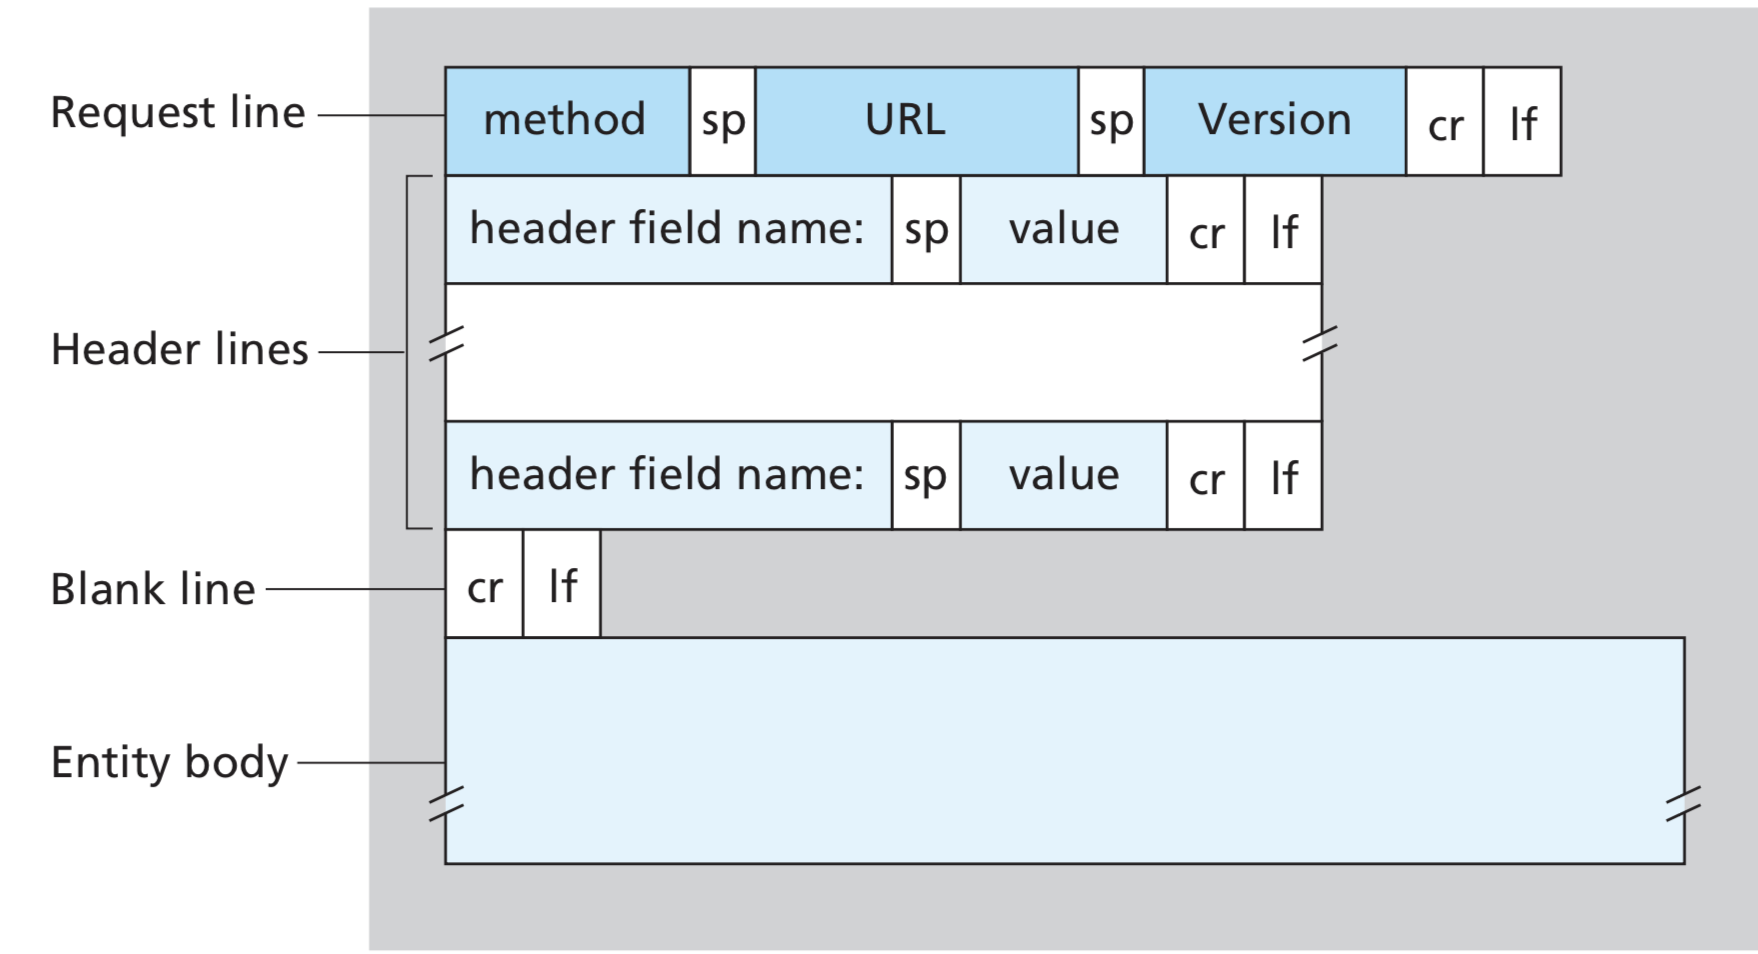
\includegraphics[scale=0.20]{http_request}}

\textbf{DNS}
\begin{itemize}[leftmargin=*]
\item DNS (Domain Name Server) holds Resource Records (RR)
  \begin{itemize}[leftmargin=*]
  \item (Name, Value, Type, TTL)
  \item \texttt{Type=A} $\Rightarrow$ Name: hostname, Value: IP
  \item \texttt{Type=NS} $\Rightarrow$ Name: domain, Value: IP of authoritative DNS
  \item \texttt{Type=CNAME} $\Rightarrow$ Name: alias hostname, Value: canonical hostname
  \item \texttt{Type=MX} $\Rightarrow$ Name: alias hostname, Value: canonical name of mail server
  \end{itemize}
\item Root servers direct queries to TLD servers, only ~13 root servers in the world
\item TLD (Top-level Domain) responsible for \texttt{.com, .org, .net, .sg...}
\item Authoritative server keeps hostname-IP mappings of organization's named hosts
\item Local DNS acts as a proxy, caches previously retrieved mappings to cache. This allows for faster lookup. Owned by ISPs
\item All DNS servers can implement caching, so root servers are often not called upon
\item DNS uses port 53
\end{itemize}

\textbf{DELAY}
\begin{itemize}[leftmargin=*]
\item There are four types of delays:
  \begin{itemize}[leftmargin=*]
  \item N (Number of Bits to Transmit)
  \item Transmission Delay $(d_{trans})$ : N / Transmission Rate
  \item Propogation Delay $(d_{prop})$: distance / Propogation Speed
  \item Queing Delay $(d_{queue})$: Time spent in Queue at Router R
  \item Processing Delay $(d_{process})$: Time spent to process by Router R
  \end{itemize}
\item RTT (Round-Trip-Time): $d_{prop} + d_{queue} + d_{process}$
\item Throughput (End to End delay): $N / (d_{trans} + d_{prop} + d_{queue} + d_{process})$
\item Link Utilization: $d_{trans} / (d_{trans} + RTT)$
\end{itemize}

% TRANSPORT LAYER %
{\small\textbf{Transport Layer}} \\
\textbf{In general}
\begin{itemize}[leftmargin=*]
\item Provides logical communication between \texttt{processes} by sending \texttt{segments}
\item Note that the term \texttt{datagram} is used for Network layer, but is commonly used to refer to UDP packets as well
\item The end goal of TCP/UDP is to extend host-to-host delivery to process-to-process delivery (transport-layer multiplexing and demultiplexing)
\end{itemize}

\textbf{RDP}
\begin{itemize}[leftmargin=*]
\item Checksum implemented if channel can flip bits (2.0)
\item ACK/NAK used to recover from bit errors (2.0)
\item ACK/NAK used to recover from bit errors (2.0)
\item Sequence number used to account for ACK/NAK corruption (2.1)
\item ACK$0/1$ used instead of NAK (2.2) for simplicity
\item Timeout added to account for packet loss (but not reordered) (3.0)
\end{itemize}

\textbf{Pipelining}
\begin{itemize}[leftmargin=*]
\item Go-Back-N:
  \begin{itemize}[leftmargin=*]
  \item Receiver sends cumulative ACK $\Rightarrow$ all packets $\leq$ $n$ have been received $\Rightarrow$ ensures order
  \item Receiver discards any packets not in order
  \item Sender attaches $k$-bits sequence to packet header $\Rightarrow$ can represent at least $[0, n]$
  \item Sliding window of size $n$ is kept
  \item Keep timer for oldest unACKed packet
  \item Resend all $n$ packets in window on timeout
  \end{itemize}
\item Selective Repeat:
  \begin{itemize}[leftmargin=*]
    \item Receives acknowledges packets individually
    \item Receives buffers out-of-order packets for eventual in-order delivery (to upper layer 
    \item Sender maintains timer for each unACKed packet $\Rightarrow$ only retransmit that packet on timeout
    \item Sender attaches $k$-bits sequence to packet header $\Rightarrow$ can represent at least $[0, n]$
    \item Sliding window of size $n$ is kept
    \item Keep timer for oldest unACKed packet
    \item Resend all $n$ packets in window on timeout
  \end{itemize}
\end{itemize}

\textbf{UDP}
\begin{itemize}[leftmargin=*]
\item User creates a socket to send segment, and specifies IP address and port \# in the segment
\item Receiver checks destination port in segment, and redirects to the socket with that port number
\item Benefits:
  \begin{itemize}[leftmargin=*]
  \item No connection set-up
  \item No state to remember
  \item Small header size $\Rightarrow$ less overhead
  \item No congestion control (as compared to TCP)
  \item Checksum to verify integrity
  \end{itemize}
\item Checksum value included in UDP checksum field. Example checksum:
  \begin{itemize}[leftmargin=*]
  \item Split into 16bit integers
  \item Add integers, use wrap-around carry
  \item Compute 1's complement (flip all bits)
  \end{itemize}
\end{itemize}

{\centering 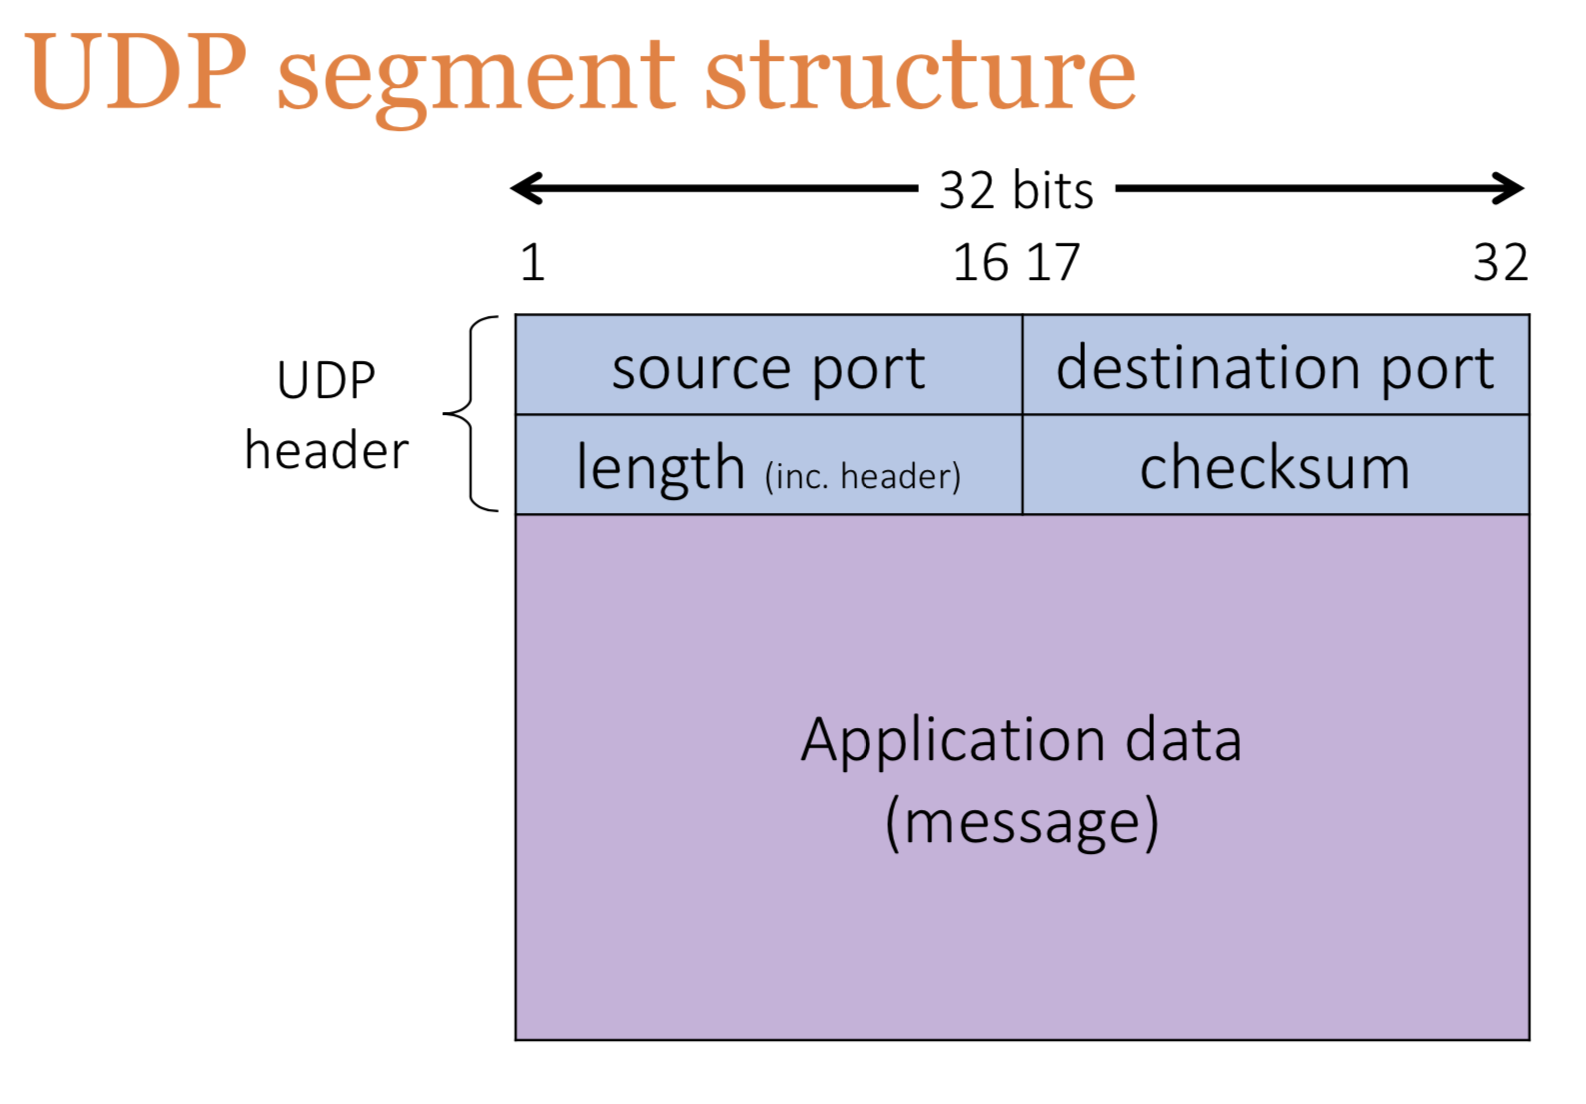
\includegraphics[scale=0.20]{udp_segment_structure}}

\textbf{TCP}
\begin{itemize}[leftmargin=*]
\item Connection-oriented -- Handshake is required before transmission
\item Reliable, in-order byte stream
\item Offset field allows for additional headers (it stores total number of TCP headers)
\item Sequence Number is byte number of first byte of data in segment
\item ACK Number is the sequence number of the next byte of data expected
\item ACK Bit represents if the ACK number should be read
\item SYN Bit initiates a connection
\item FIN Bit is to denote closing of the connection (Final)
\item RST Bit is to denote abortion of a connection due to error
\item PSH Bit is to indicate that the data should be pushed to application level immediately, without waiting for additional data
\item URG Bit is to indicate to a receiving station that the data is urgent and should be prioritised
\item Receive window tells sender how much data can be sent
\item Timeout:
  \begin{itemize}[leftmargin=*]
  \item Too long $\Rightarrow$ slow reaction to loss
  \item Too short $\Rightarrow$ Premature timeout and unnecessary retransmissions
  \item Estimate RTT using Exponential Weighted Moving Average: $RTT_E = (1 - a) * RTT_E + a * RTT_s$, where $a$ is usually $\frac{1}{8}$
  \item Calculate deviation of RTT using $RTT_{dev} = (1 - b) * RTT_{dev} + b*RTT_s - RTT_E$, where $b$ is usually $\frac{1}{4}$
  \item Retransmission Timeout is $RTO = RTT_{E} + 4 * RTT_{dev}$, the deviation is used as a "safety margin"
  \item Note that the RTO is \textbf{doubled} after each timeout
  \item TCP Fast transmission: If 3 Duplicate ACK
  \end{itemize}
\end{itemize}

{\centering 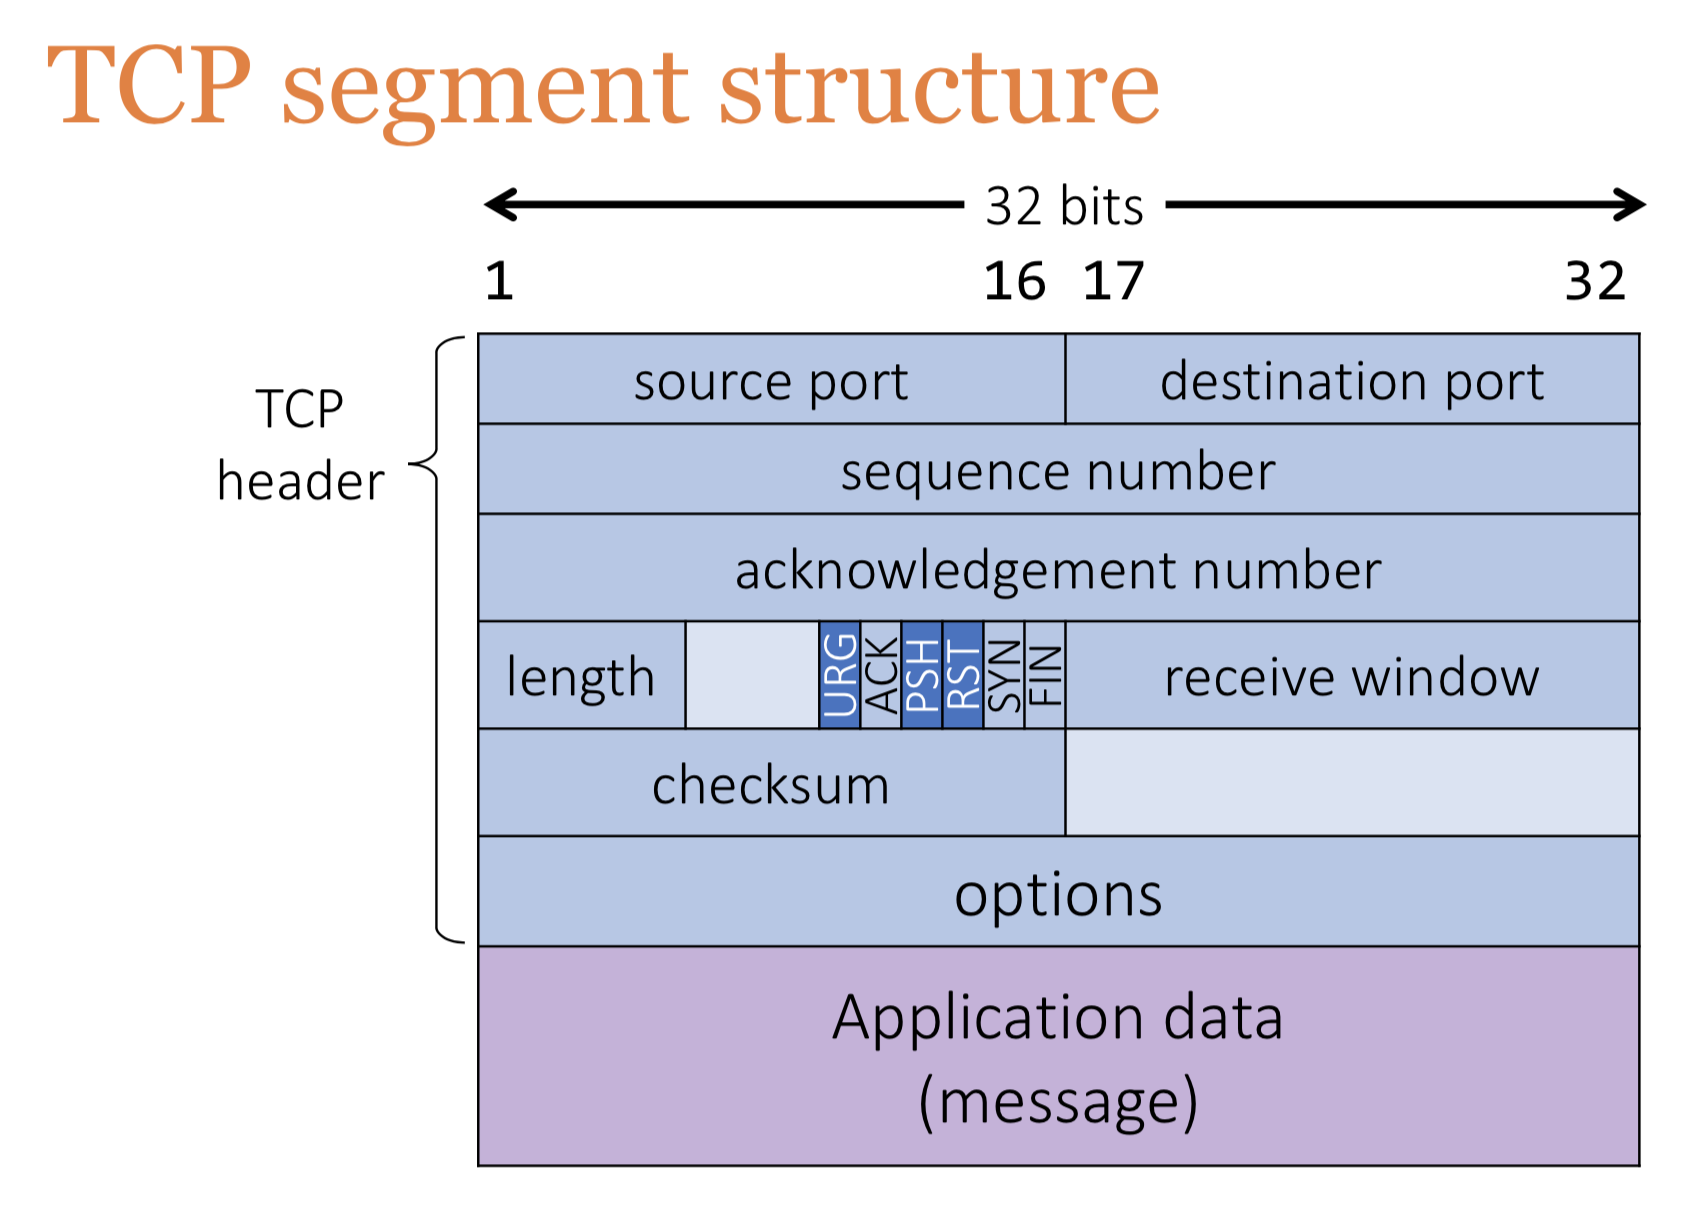
\includegraphics[scale=0.20]{tcp_segment_structure}}
{\centering 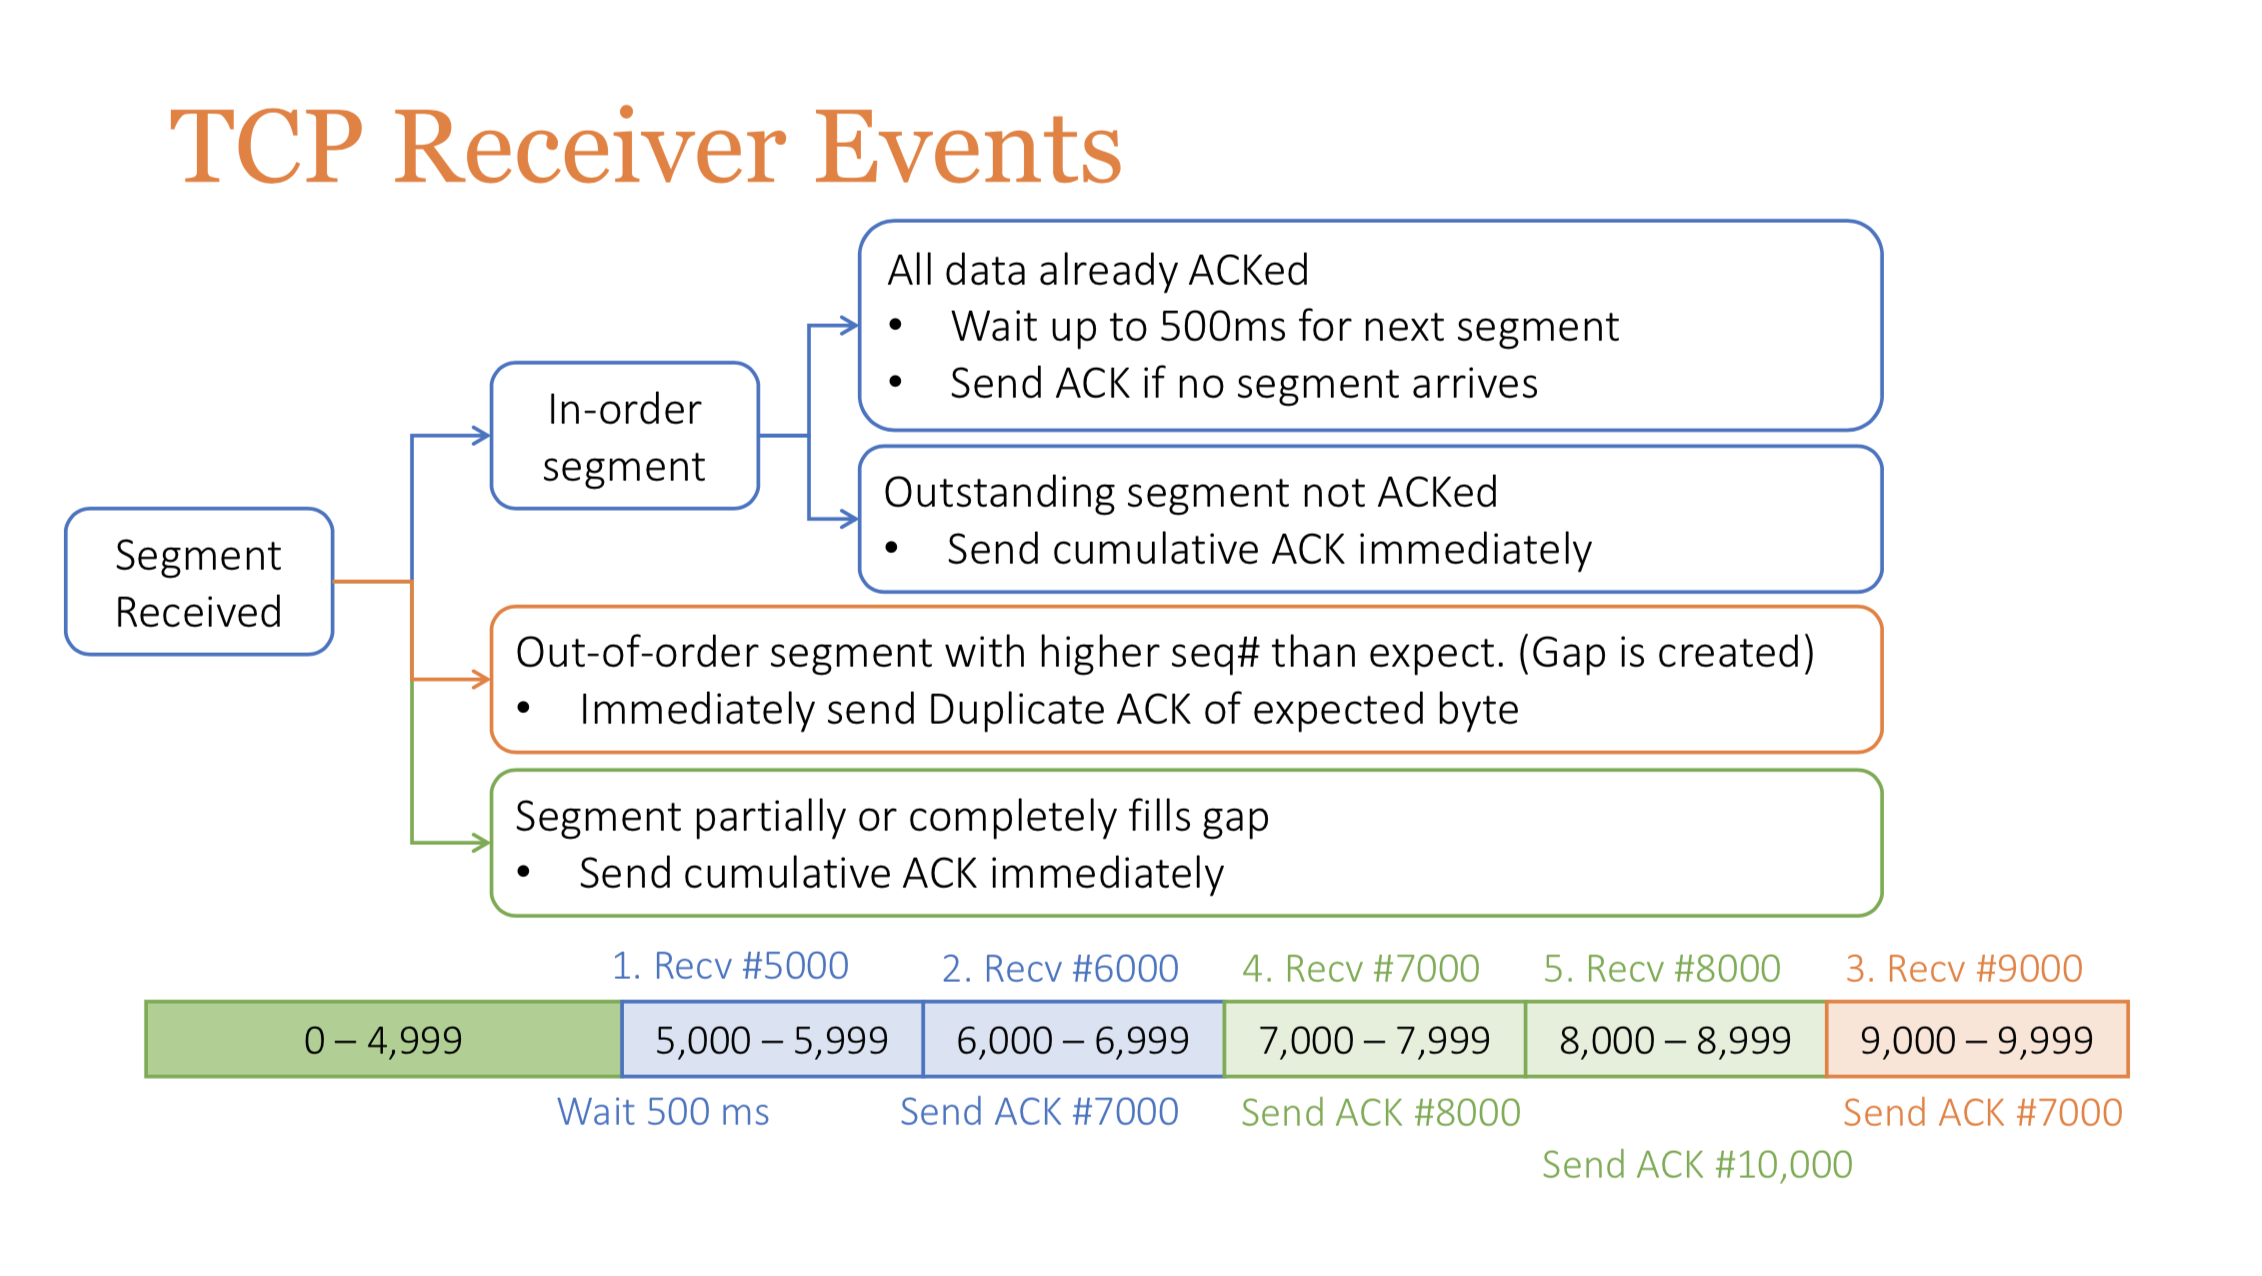
\includegraphics[scale=0.18]{tcp_receiver_events}}

% NETWORK LAYER %
{\small\textbf{Network Layer}} \\
\textbf{In general}
\begin{itemize}[leftmargin=*]
\item Provides logical communication between \texttt{hosts}, through \texttt{routers}
\item Has two responsibilities: \texttt{forwarding} (through a single output link) and \texttt{routing} (determining the route that packets should follow)
\end{itemize}

\textbf{IP}
\begin{itemize}[leftmargin=*]
\item IP Address is 32bit
\item IP Address is associated with an interface e.g 802.11 wifi
\item However, the device that we call "router", actually forwards packets between networks. This device has multiple interfaces e.g LAN ports are all one interface
\item Dynamic Host Configuration Protocol:
  \begin{itemize}[leftmargin=*]
  \item Host broadcast a $Discover$ message
  \item DHCP server (listening on port 67) reponds with an offer. First transaction ends here.
  \item Host requests for the given IP with a new Transaction (new transaction ID used)
  \item DHCP ACKnowledges request and assigns the IP
  \end{itemize}
\item Some IP Addresses are reserved
\item Hierarchical addressing scheme:
  \begin{itemize}[leftmargin=*]
  \item IP Addresses grouped into subnets, each subnet having a certain prefix for all IP Addresses
  \item Internet decides which ISP to send the packet to using the Longest Prefix of the address
  \item Subnet mask is a common prefix used between hosts in the same subnet, where they can communicate between each other without a router
  \end{itemize}
\item Network Address Translation:
  \begin{itemize}[leftmargin=*]
  \item Entire subnet under the router is identified by a single IP Address
  \item NAT translation table used to map $(IP_{subnet}, port)$ to $(IP_{global}, port)$
  \item Hosts' identities are effectively "firewalled" from the outside world
  \item External parties cannot identify hosts using IP, only using port (which is supposed to be used on the Application-level)
  \end{itemize}
\end{itemize}

{\centering 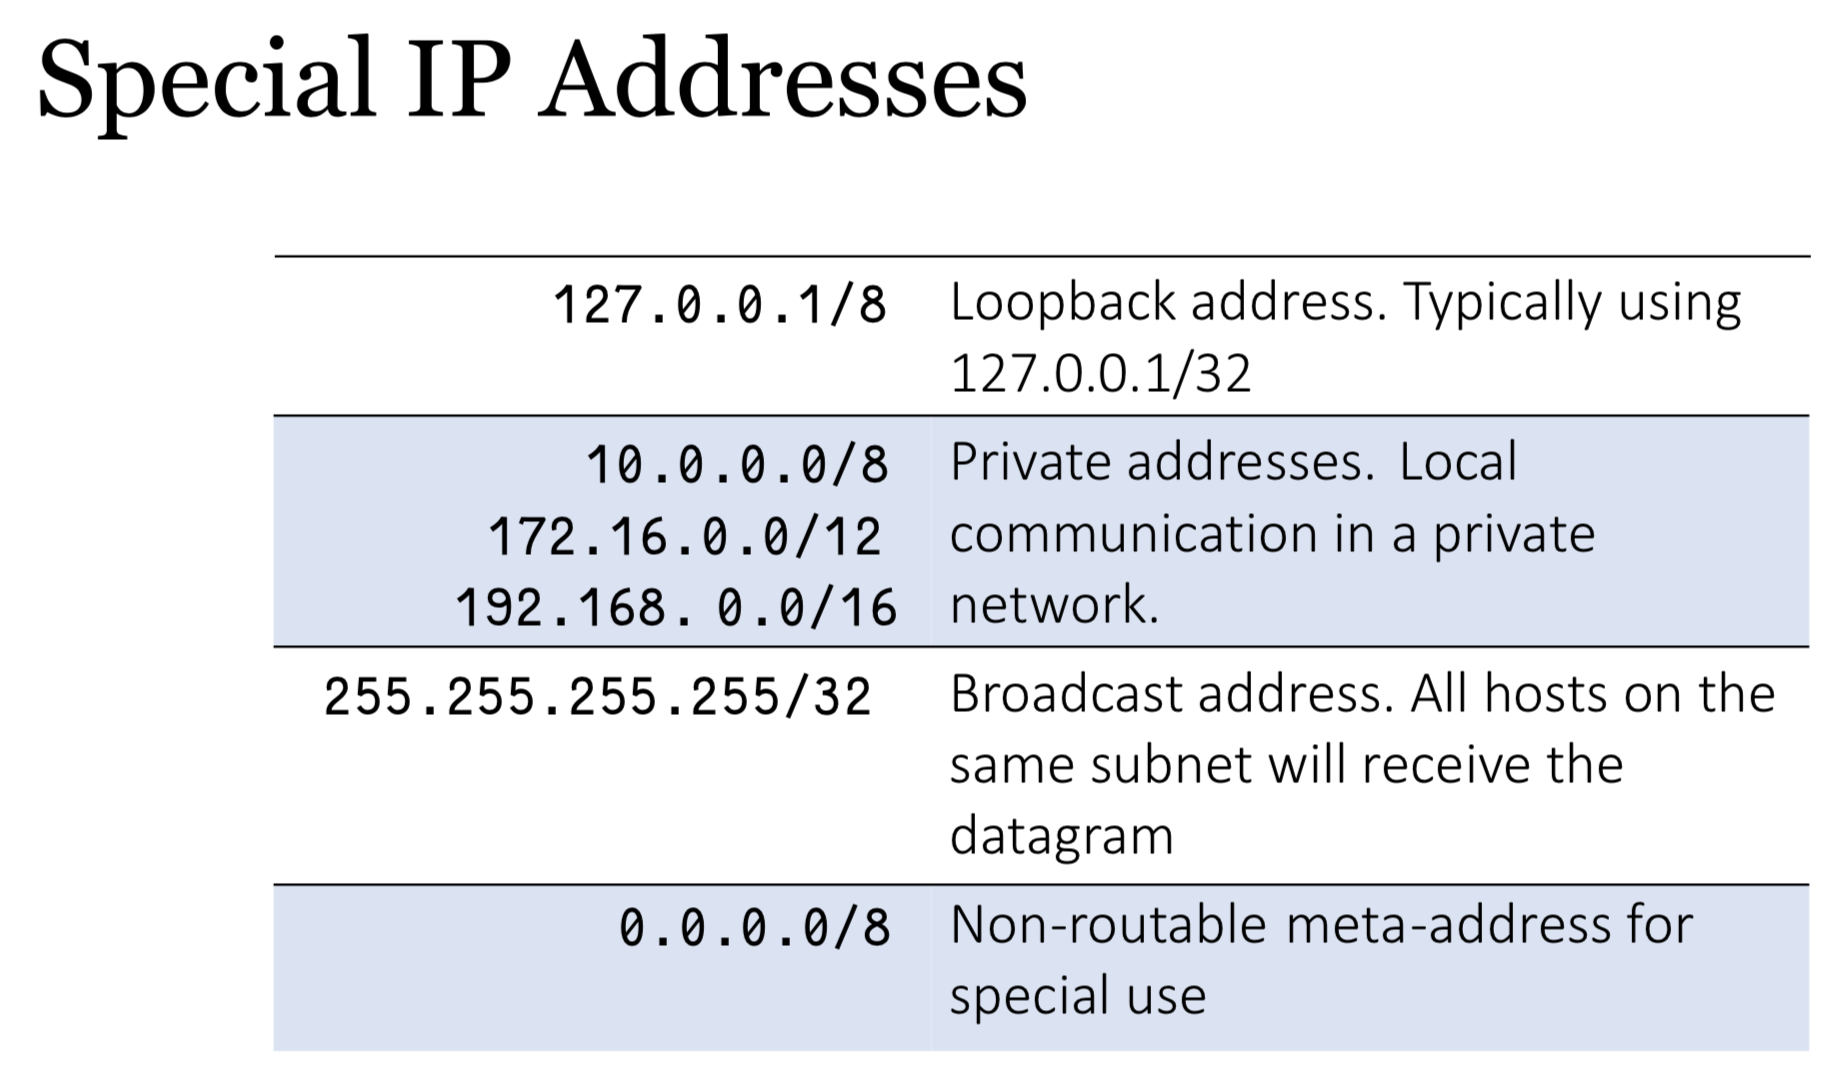
\includegraphics[scale=0.17]{special_ip_addresses}}
{\centering 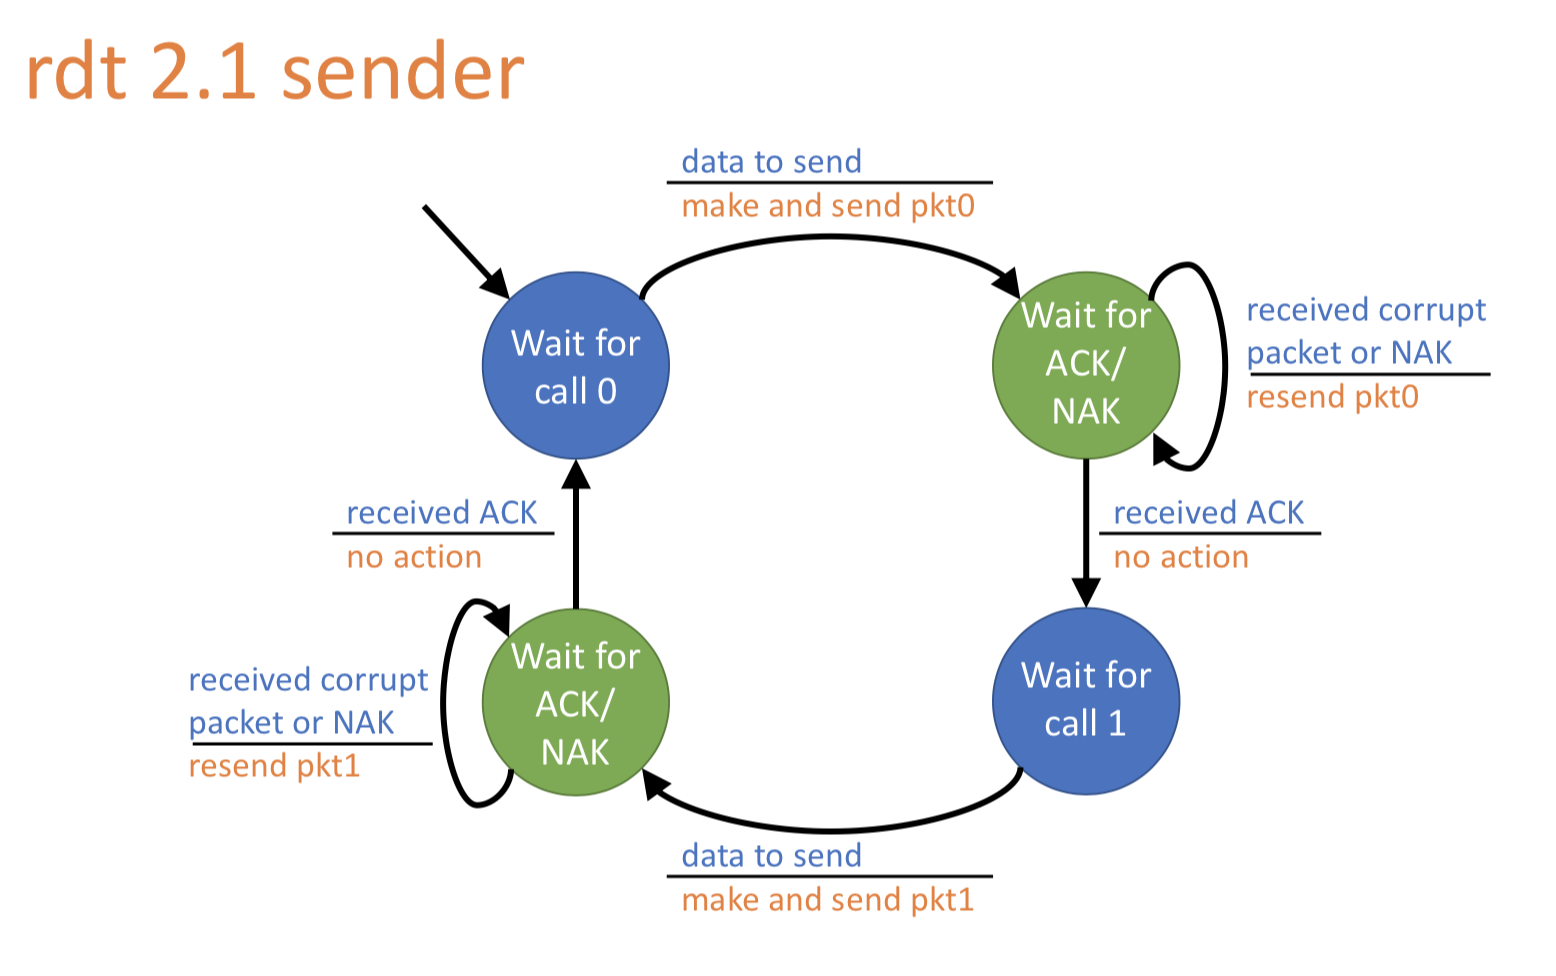
\includegraphics[scale=0.27]{rdt_2_1_sender}}
{\centering 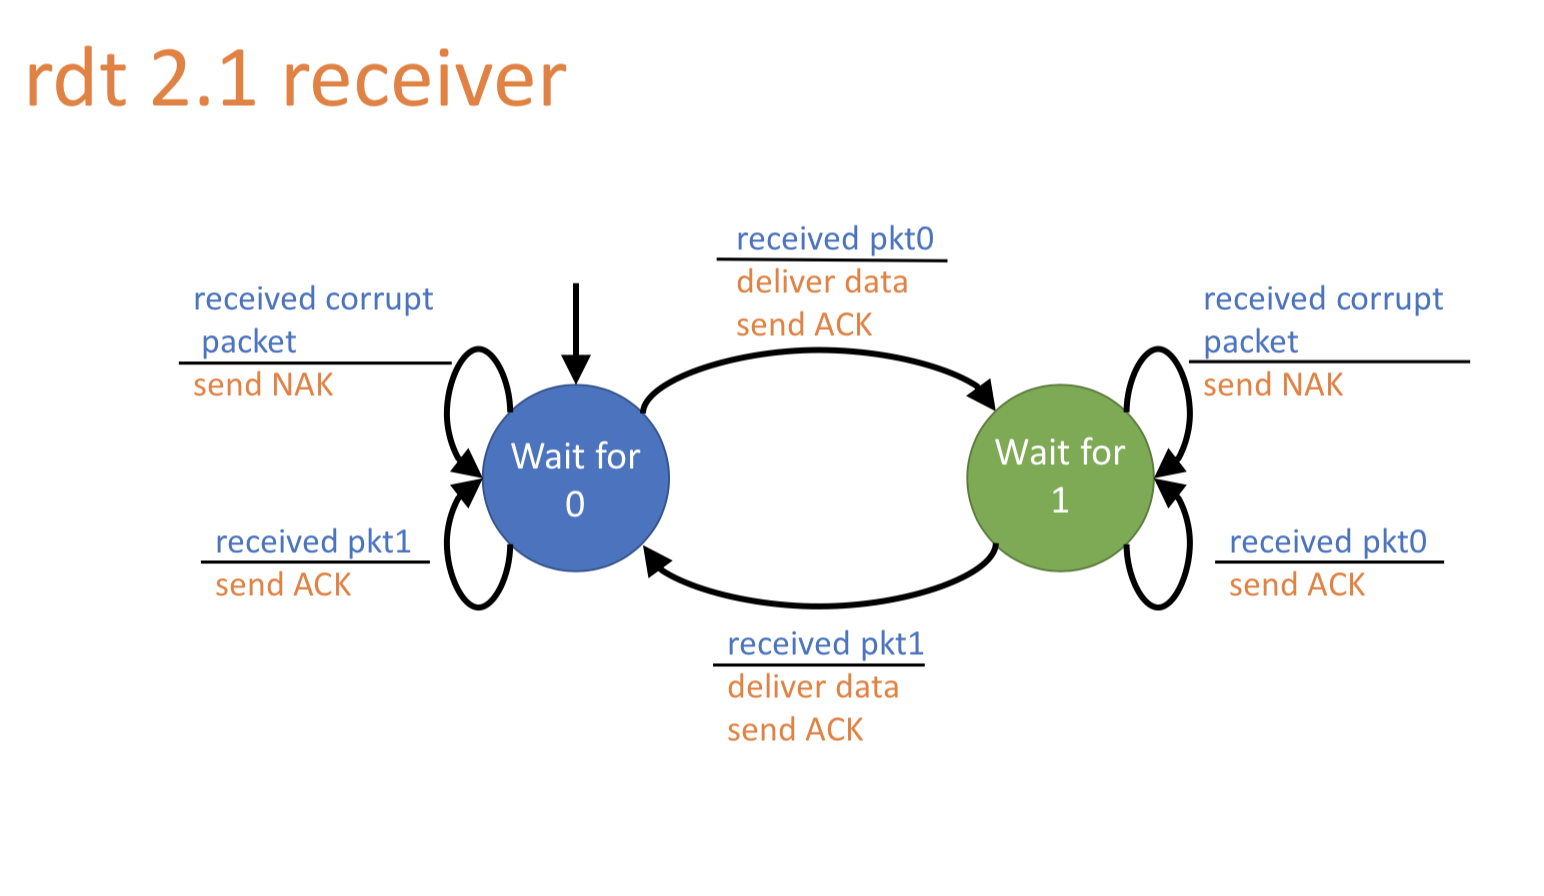
\includegraphics[scale=0.27]{rdt_2_1_receiver}}
{\centering 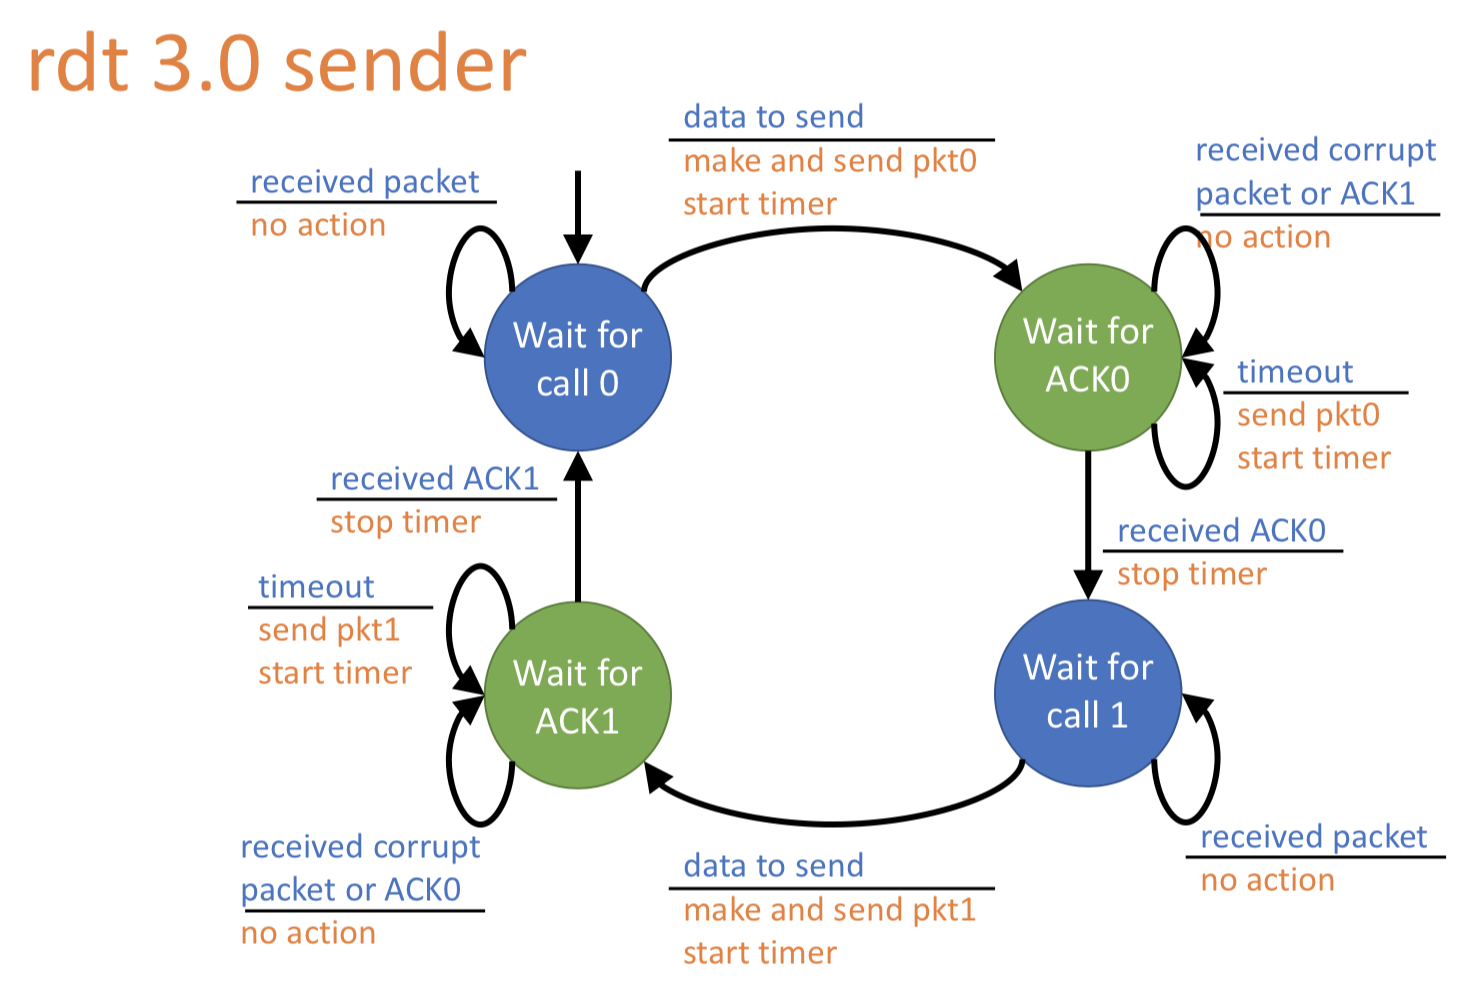
\includegraphics[scale=0.27]{rdt_3}}

\textbf{Java Socket Programming}

{\centering 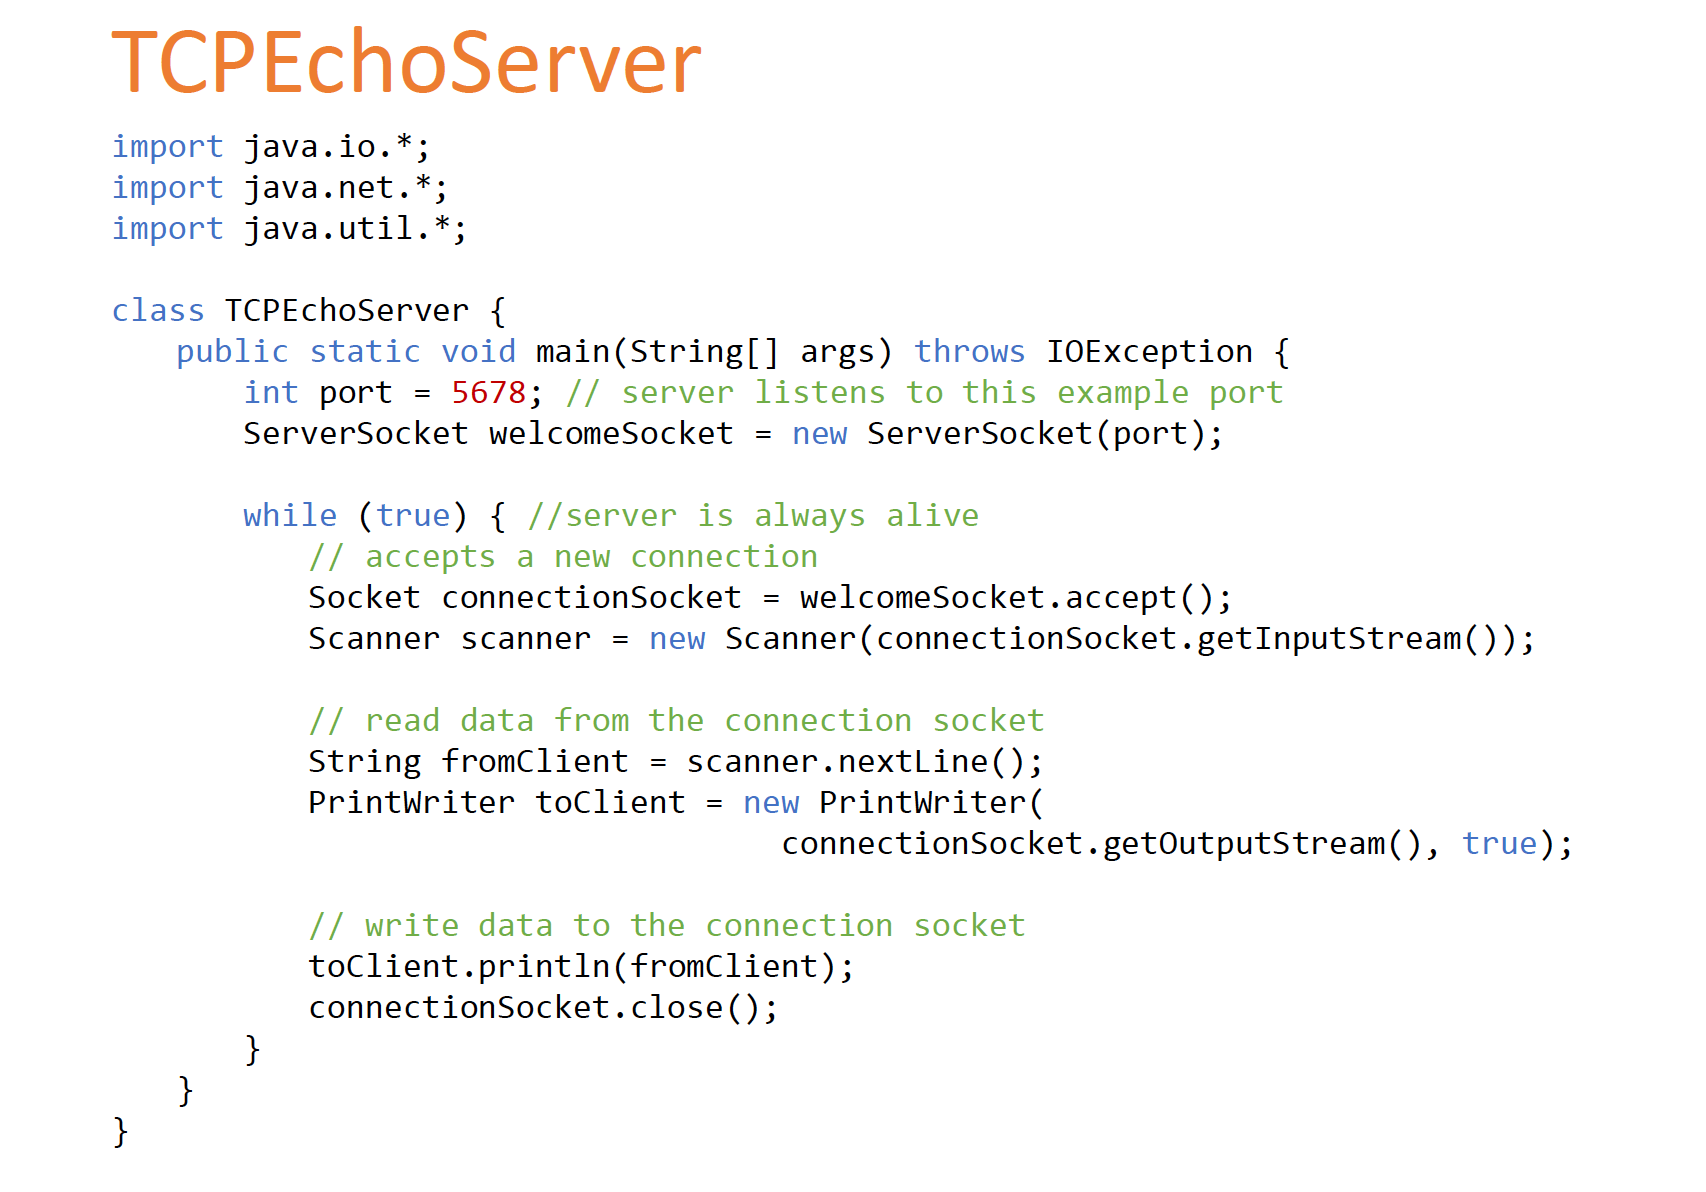
\includegraphics[scale=0.17]{TCPEchoServer}}

{\centering 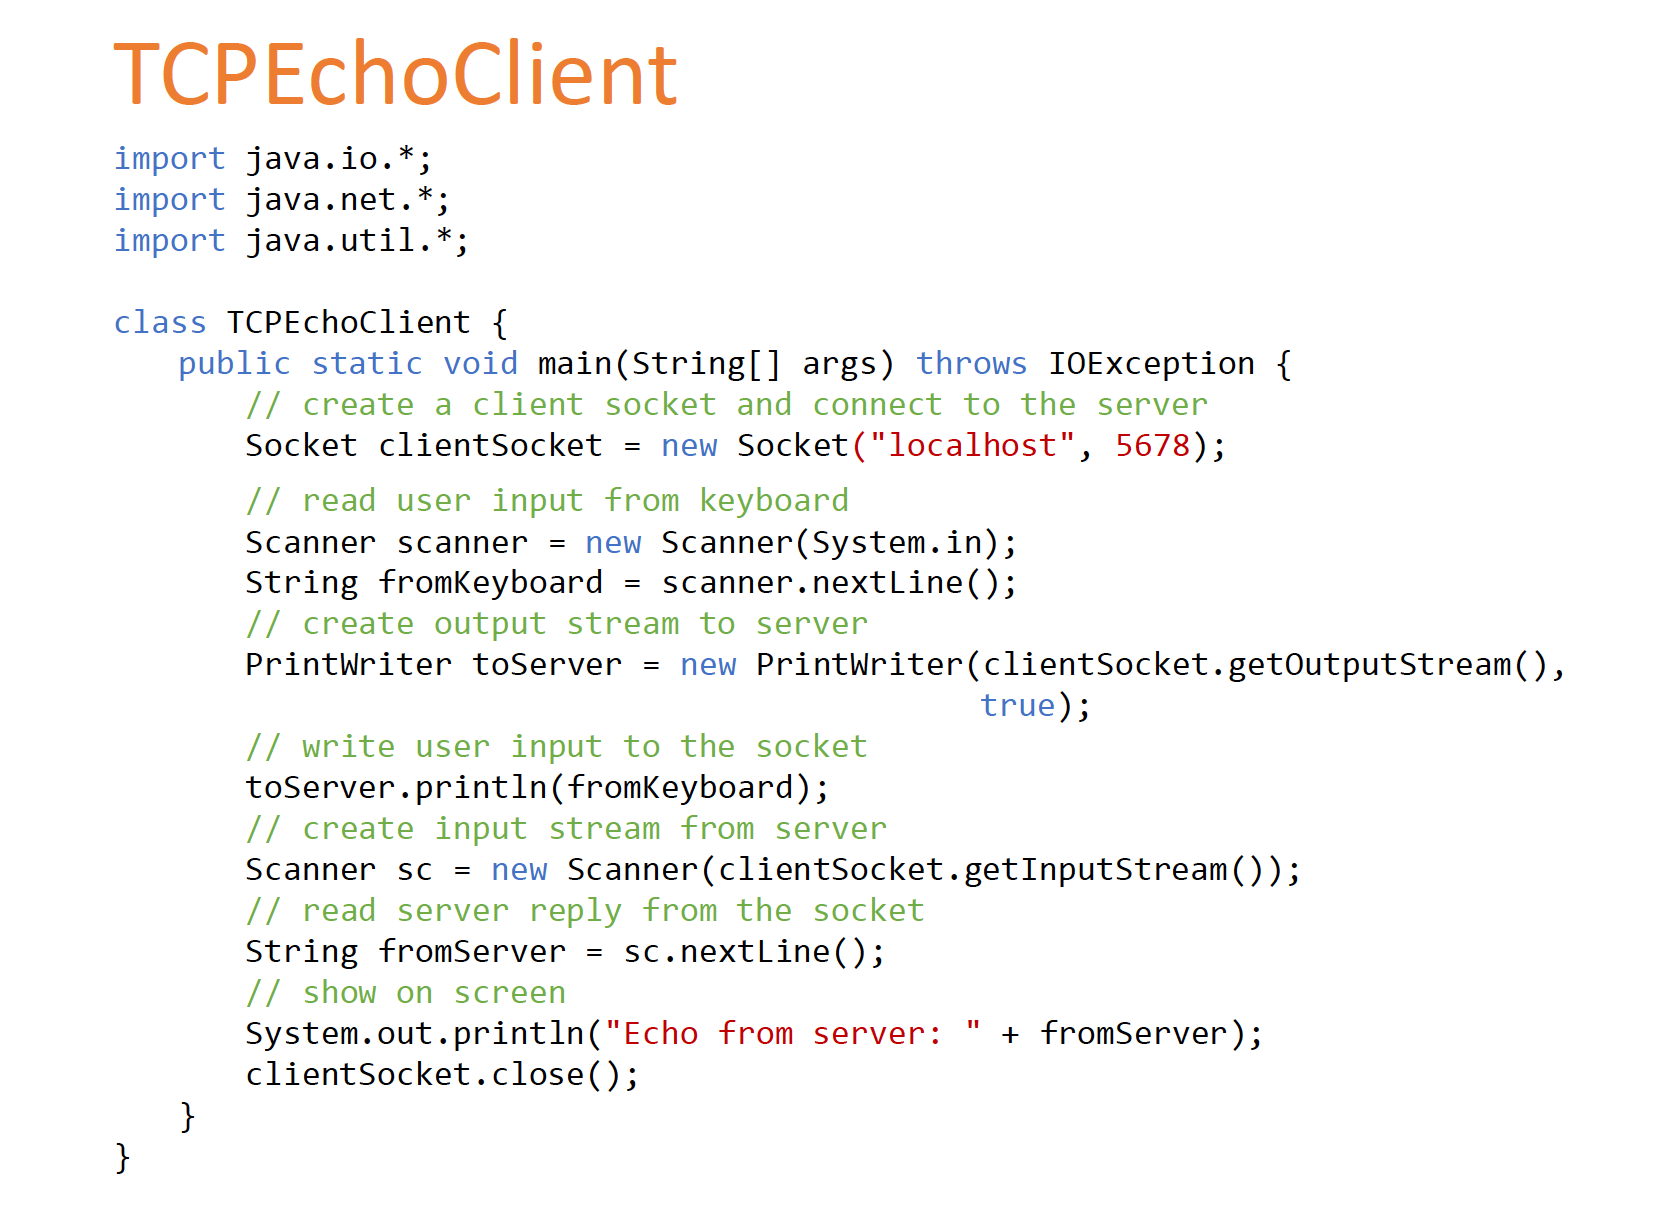
\includegraphics[scale=0.17]{TCPEchoClient}}

    \end{multicols*}
\end{document}
